\section{Laboratory work implementation}

\subsection{Tasks and Points}


Advanced Level:
	-Add 2 animated objects which will interact with each other. Balls that have different velocity and moving angles. They should behave based on following rules:
	-At the beginning you should have 3 balls of different colours of the same size
	-On interaction with each other, if they are of the same class (circle, square), they should 		change their color and be multiplied.
	-On interaction with the right and left wall (the margins of the window), they should be 			transformed into squares.
	-On interaction with the top and bottom of the window - the figures should increase their 			velocity.
	-Please, take into consideration that the user can increase and decrease animation speed using 	mouse wheel/from keyboard

\subsection{Laboratory work analysis}

Repository:

https://github.com/VictorIstratii151/WP-labs

\subsection{Proving my work}

The one thing is annoying about  win32 api -- when it comes to implement continuous animations of different objects, but more precisely when you draw directly to the HDC of your window, there is a big possibility that the screen will be updated before the drawing is finished. That's why usually there occur strange graphical artefacts, known as flickers. The more drawing operations are performed, the messier looks the screen.

The solution to this problem is pretty easy and is called Double Buffering. This means that we just do all our drawing in memory first, and then copy the completed drawing to the screen, using a single BitBlt() function. That results in the screen getting updated directly from the old image.

To do this, we create a temporary HBITMAP in memory that is the exact size of the area we are going to draw to the screen. We also need a HDC so that we can BitBlt() to the bitmap.

Then, having a place to draw to in memory, all of the drawing operations use a buffer instead of window's hdc, meaning that the results are stored in memory until they are complete.

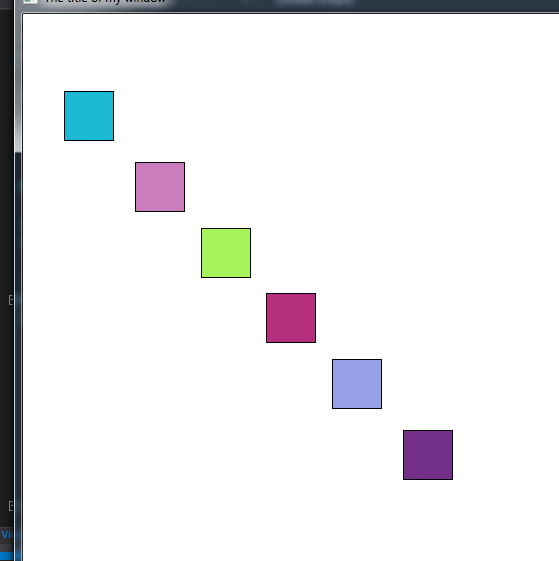
\includegraphics{im1}
At first we see that on the screen are created only squares.

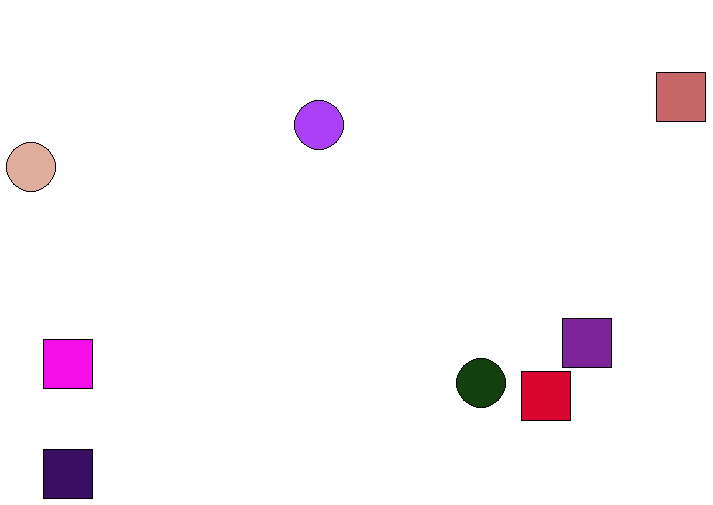
\includegraphics{im2}
Observe that, after some interactions, several squares are transformed to balls.



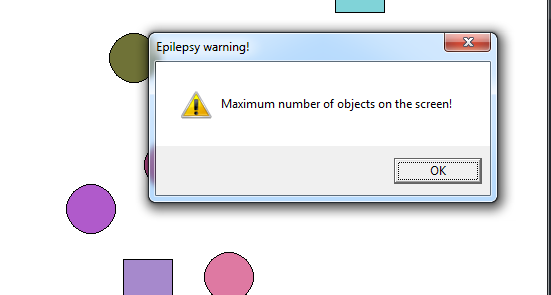
\includegraphics{im3}
When objects on the screen are too much, we can't add any more, so it is issued an error. 



\clearpage